\chapter{PmodCLP}

Der PmodCLP besteht aus einem Samsung KS0066 LCD Controller und einem Sunlike LCD Panel, worüber Informationen dargestellt werden können {lcd-desc}. Es ist möglich 32 Positionen auf dem 16x2 LCD Panel zu nutzen. Pro Position werden die Zeichen dabei mit einer Auflösung von 5x8 angezeigt. \newline

Das System besteht im Wesentlichen aus drei Komponenten. Der character-generator ROM (CGROM) hält 192 vordefinierte Zeichen, darunter 93 ASCII Charaktere. Anschaulich gesehen können die Zeichen über eine matrixartige Struktur indiziert werden, welche im Datenblatt festgelegt ist. Neben den nicht-volatilen Daten im CGROM ist es möglich bis zu 8 eigene Zeichen volatil im character-generator RAM (CGRAM) zu halten. Um nun Zeichen aus diesen beiden Repositories auf dem Panel anzeigen zu können, gibt es den data RAM (DDRAM). Hier können bis zu 80 Zeichencodes gespeichert werden. Er fungiert als Indexspeicher für Daten innerhalb des CGROM oder CGRAM. Wird ein Index aus der matrixartigen Struktur in den DDRAM geladen, erscheint das entsprechende Zeichen auf dem Display. \newline

Das Display selbst verfügt über 2 Zeilen á 16 Positionen. Insgesamt stehen jedoch nicht 32 Speicherplätze zur Verfügung, sondern 39, um beispielsweise Scrolling zu verwenden. \newline

Wichtige Schnittstellen des Samsung KS0066 LCD Controller sind

\begin{itemize}
    \item \textit{DB4-DB7}: Datenbits im Nibble-Mode zur Codierung von Befehlen/Zeichen
    \item \textit{RS (Register Select)}: High für Daten, Low für Instruktionen
    \item \textit{RW (Read/Write)}: High = Read, Low = Write
    \item \textit{E (Enable)}: High für Read, Falling Edge für Write
\end{itemize}

Um diese nutzen zu können wird folgendes Mapping auf dem FPGA hinterlegt:\newline

\begin{lstlisting}[language=bash,caption={Pin-Zuordnung im Constraints-File},breaklines=true,captionpos=b,basicstyle=\footnotesize\ttfamily,
    label={lst:fpga_pins}]
set_property -dict {PACKAGE_PIN D13 IOSTANDARD LVCMOS33}[get_ports{clp_db_tri_io[4]}];#db04
set_property -dict {PACKAGE_PIN B18 IOSTANDARD LVCMOS33}[get_ports{clp_db_tri_io[5]}];#db05
set_property -dict {PACKAGE_PIN A18 IOSTANDARD LVCMOS33}[get_ports{clp_db_tri_io[6]}];#db06
set_property -dict {PACKAGE_PIN K16 IOSTANDARD LVCMOS33}[get_ports{clp_db_tri_io[7]}];#db07
set_property -dict {PACKAGE_PIN E2 IOSTANDARD LVCMOS33}[get_ports{clp_cb_tri_o[0]}];  #lcd_rs
set_property -dict {PACKAGE_PIN D2 IOSTANDARD LVCMOS33}[get_ports{clp_cb_tri_o[1]}];  #lcd_rw
set_property -dict {PACKAGE_PIN H2 IOSTANDARD LVCMOS33}[get_ports{clp_cb_tri_o[2]}];  #lcd_e
\end{lstlisting}

Die Zuordung in Aufzählung \ref{lst:fpga_pins} greift auf zwei Header des PmodCLP-Boards zurück. Die Daten-Bits db04-db07 sind an die untere Hälfte des Headers J1 gebunden. Die Steuersignale Register Select, Read/Write und Enable hingegen an Header J2.

\section{Ansatz Custom IP}

Im ersten Schritt soll die IP funktional fertiggestellt werden. Sie soll dabei mittels Polling eingesetzt werden. Sobald die Funktionalität des Gesamtsystems vollumfänglich gegeben ist, wird anstatt Polling über eine AXI Schnittstelle kommuniziert.\newline

Das Projektteam hat sich auf folgenden Entwurf geeinigt:

\begin{itemize}
    \item \textit{Submodul 1}: Finite-State-Machine (FSM) \newline
    Mittels einer FSM wird aus den Registern, welche von Microprozessor gesetzt werden können, der Befehl interpretiert.
    \item \textit{Submodul 2}: Init/Reset \newline
    Für die Initialisierung bzw. Reset müssen diverse Zeitbedinungen eingehalten werden.\newline
    \begin{figure}[h!]
        \centering
        \begin{minipage}{0.15\textwidth}
            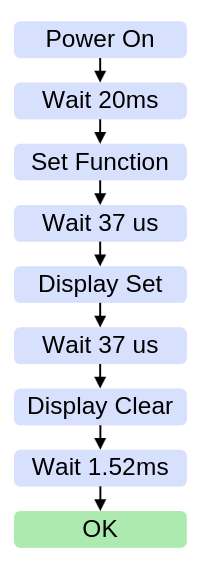
\includegraphics[width=\linewidth]{./images/lcd_timing.png} % replace with your image filename
        \end{minipage}
        \caption{Startup Sequence}
        \label{fig:startup_sequence}
    \end{figure}
    Die Graphik \ref{fig:startup_sequence} stellt die verschiedenen Schritte während des Starts dar. Erst nach 21.594ms ist es möglich, Daten in den DDRAM zu schreiben.
    \item \textit{Submodul 3}: ASCII zu Zeichencode CGROM/CGRAM
    \item \textit{Submodul 4}: DDRAM Adressierung
    \item \textit{Submodul 4}: PmodCLP Kommunikation
\end{itemize}

TODO

\begin{itemize}
    \item Set Function: Busbreite, Zeilenanzahl, Zeichenmuster konfigurieren
    \item Display Set: Display anschalten, Cursor an-/ausschalten, Cursor-Blinken konfigurieren
    \item Entry Mode Set: Adress-Inkrement/ -Dekrement, Display-Shift aktivieren/deaktivieren
\end{itemize}

Danach können Daten ins DDRAM geschrieben werden, um Informationen anzuzeigen.

\section{Registermapping}

\subsection{I/Os}
\begin{longtable}{|p{2.5cm}|p{1cm}|p{2cm}|p{9cm}|}
\hline
\textbf{Signal Name} & \textbf{I/O} & \textbf{Initial State} & \textbf{Description} \\
\hline
ap\_clk(s00\_axi\_aclk) & I & NA & AXI Clock \\
\hline
ap\_rst\_n (s00\_axi\_aresetn) & I & NA & AXI Reset, active-Low \\
\hline
s\_axi\_control* (s00\_axi*) & NA & NA & AXI4-Lite Slave Interface signals \\
\hline
interrupt & O & 0x0 & Indicates that the condition for an interrupt on this timer has occurred. (timer rolled over)
\newline 0 = No interrupt has occurred
\newline 1 = Interrupt has occurred \\
\hline
o\_t0\_out & O & 0x0 & Timer generated blinking for led (timer rolled over condition toggles signal) \\
\hline
\caption{PmodCLP Überblick I/O}
\end{longtable}

\subsection{Registerbereich}
\begin{longtable}{|p{3cm}|p{4cm}|p{7cm}|}
\hline
\textbf{Address Offset} & \textbf{Register Name} & \textbf{Description} \\
\hline
0x00 & GCSR & General/Global Control and Status Register \\
\hline
0x04 & GIER & Global Interrupt Enable Register \\
\hline
0x08 & IPIER & IP Interrupt Enable Register \\
\hline
0x0C & IPISR & IP Interrupt Status Register (Interrupt Pending) \\
\hline
0x10 & IDR & ID Register \\
\hline
0x14 & VERR & Version Register \\
\hline
0x18 & SCSR0 & Special Control and Status Register \\
\hline
0x1C & CR0 & Counter Register \\
\hline
0x20 & LR0 & Load Register \\
\hline
0x24 & reserved & reserved \\
\hline
\caption{PmodCLP Registerbereich}
\end{longtable}

\subsection{Registerbeschreibung (MSB bit31 LSB bit0)}

\subsubsection*{0x00 GCSR}
\begin{longtable}{|p{1.5cm}|p{3cm}|p{2cm}|p{2cm}|p{5cm}|}
\hline
\textbf{Bit} & \textbf{Name} & \textbf{Access Type} & \textbf{Reset Value} & \textbf{Description} \\
\hline
0 & ap\_start & R/W & 0 & Asserted when the kernel can start processing data. Cleared on handshake with ap\_done being asserted. \\
\hline
1 & ap\_done & R & 0 & Asserted when the kernel has completed operation. Cleared on read. \\
\hline
2 & ap\_idle & R & 0 & Asserted when the kernel is idle. \\
\hline
3 & reserved (ap\_ready) & R & 0 & Asserted by the kernel when it is ready to accept the new data (used only by AP\_CTRL\_CHAIN)) \\
\hline
4 & reserved (ap\_continue) & R/W & 0 & Asserted by the XRT to allow kernel keep running (used only by AP\_CTRL\_CHAIN) \\
\hline
5:6 & reserved & & & \\
\hline
7 & auto\_restart & R/W & 0 & Used to enable automatic kernel restart. This bit determines whether the counter reloads the load register value and continues running or holds at the termination value.
\newline 0 = Hold counter
\newline 1 = Reload load register value \\
\hline
31:8 & reserved & & & \\
\hline
\caption{PmodCLP Registerbeschreibung}
\end{longtable}

\subsubsection*{0x04 GIER}
\begin{longtable}{|p{1.5cm}|p{3cm}|p{2cm}|p{2cm}|p{5cm}|}
\hline
\textbf{Bit} & \textbf{Name} & \textbf{Access Type} & \textbf{Reset Value} & \textbf{Description} \\
\hline
0 & gie & R/W & 0 & When asserted, along with the IP Interrupt Enable bit, the interrupt is enabled. \\
\hline
31:1 & reserved & & & \\
\hline
\caption{PmodCLP Register GIER Details}
\end{longtable}

\subsubsection*{0x08 IPIER}
\begin{longtable}{|p{1.5cm}|p{3cm}|p{2cm}|p{2cm}|p{5cm}|}
\hline
\textbf{Bit} & \textbf{Name} & \textbf{Access Type} & \textbf{Reset Value} & \textbf{Description} \\
\hline
0 & ipie & R/W & 0 & When asserted, along with the Global Interrupt Enable bit, the interrupt is enabled. (default: uses the internal ap\_done signal to trigger an interrupt) \\
\hline
31:1 & reserved & & & \\
\hline
\caption{PmodCLP Register IPIER Details}
\end{longtable}

\subsubsection*{0x0C IPISR}
\begin{longtable}{|p{1.5cm}|p{3cm}|p{2cm}|p{2cm}|p{5cm}|}
\hline
\textbf{Bit} & \textbf{Name} & \textbf{Access Type} & \textbf{Reset Value} & \textbf{Description} \\
\hline
0 & ipis & R/W & 0 & Toggle on write. (write 1 to clear(W1C)) \\
\hline
31:1 & reserved & & & \\
\hline
\caption{PmodCLP Register IPISR Details}
\end{longtable}

\subsubsection*{0x10 IDR}
\begin{longtable}{|p{1.5cm}|p{3cm}|p{2cm}|p{2cm}|p{5cm}|}
\hline
\textbf{Bit} & \textbf{Name} & \textbf{Access Type} & \textbf{Reset Value} & \textbf{Description} \\
\hline
31:0 & ID & R & 0x8001DEEF & Distinct ID \\
\hline
\caption{PmodCLP Register IDR Details}
\end{longtable}

\subsubsection*{0x14 VERR}
\begin{longtable}{|p{1.5cm}|p{3cm}|p{2cm}|p{2cm}|p{5cm}|}
\hline
\textbf{Bit} & \textbf{Name} & \textbf{Access Type} & \textbf{Reset Value} & \textbf{Description} \\
\hline
31:0 & VER & R & 0x80001000 & Version \\
\hline
\caption{PmodCLP Register VERR Details}
\end{longtable}

\subsubsection*{0x18 SCSR0}
\begin{longtable}{|p{1.5cm}|p{3cm}|p{2cm}|p{2cm}|p{5cm}|}
\hline
\textbf{Bit} & \textbf{Name} & \textbf{Access Type} & \textbf{Reset Value} & \textbf{Description} \\
\hline
0 & reserved (ENALL) & R/W & 0 & ap\_start is used Enable All Timers
\newline 0 = No effect on timers
\newline 1 = Enable all timers (counters run)
\newline This bit is mirrored in all control/status registers and is used to enable all counters simultaneously.
\newline Writing a 1 to this bit sets ENALL, EN0, and EN1.
\newline Writing a 0 to this register clears ENALL but has no effect on EN0 and EN1. \\
\hline
1 & reserved (en0) & R/W & 0 & ap\_start is used Enable Timer 0
\newline 0 = Disable timer (counter halts)
\newline 1 = Enable timer (counter runs) \\
\hline
2 & ent0\_out & R/W & 0 & Enable external pin t0\_out
\newline 0 = Disable
\newline 1 = Enable \\
\hline
3 & reserved & & & \\
\hline
4 & load0 & R/W & 0 & Load Timer 0
\newline 0 = No load
\newline 1 = Loads timer with value in LR0
\newline Setting this bit loads counter register (CR0) with a specified value in the load register (LR0).
\newline This bit prevents the running of the timer/counter; hence, this should be cleared alongside setting Enable Timer/Counter (EN0) bit. \\
\hline
5 & ud0 & R/W & 0 & Up/Down Count Timer 0
\newline 0 = Timer functions as up counter
\newline 1 = Timer functions as down counter \\
\hline
6 & reserved & & & \\
\hline
7 & reserved & & & \\
\hline
8 & reset\_ip & R/W & 0 & Stops the whole IP and resets all values \\
\hline
9 & freeze\_ip & R/W & 0 & Stops the whole IP but does not reset the values (useful for debugging) \\
\hline
10 & reserved & & & \\
\hline
11 & reserved & & & \\
\hline
31:12 & reserved & & & \\
\hline
\caption{PmodCLP Register SCSR0 Details}
\end{longtable}

\subsubsection*{0x1C CR0}
\begin{longtable}{|p{1.5cm}|p{3cm}|p{2cm}|p{2cm}|p{5cm}|}
\hline
\textbf{Bit} & \textbf{Name} & \textbf{Access Type} & \textbf{Reset Value} & \textbf{Description} \\
\hline
31:0 & CR0 & R & 0x0 & Counter Register 0 \\
\hline
\caption{PmodCLP Register CR0 Details}
\end{longtable}

\subsubsection*{0x20 LR0}
\begin{longtable}{|p{1.5cm}|p{3cm}|p{2cm}|p{2cm}|p{5cm}|}
\hline
\textbf{Bit} & \textbf{Name} & \textbf{Access Type} & \textbf{Reset Value} & \textbf{Description} \\
\hline
31:0 & LR0 & R/W & 0x0 & Load Register 0 \\
\hline
\caption{PmodCLP Register LR0 Details}
\end{longtable}